\documentclass[tikz,border=10pt]{standalone}
\begin{document}
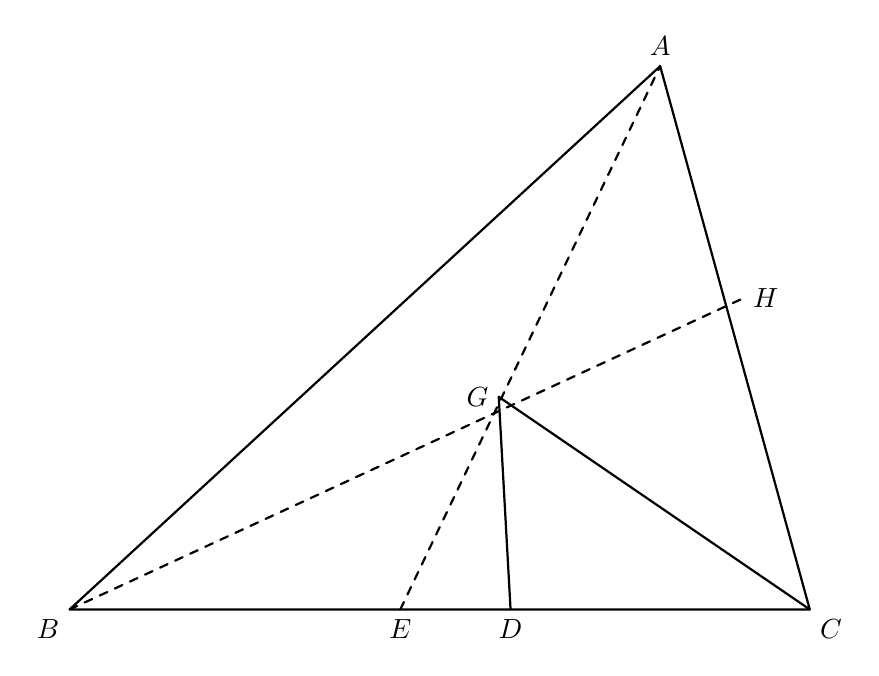
\begin{tikzpicture}[line cap=round,line join=round,thick]

\coordinate (B) at (0,0);
\coordinate (E) at (4.2,0);
\coordinate (D) at (5.6,0);
\coordinate (C) at (9.4,0);
\coordinate (G) at (5.45,2.7);
\coordinate (A) at (7.5,6.9);
\coordinate (H) at (8.55,3.95);

\draw (B) -- (A) -- (C) -- (B);
\draw (G) -- (D);
\draw (G) -- (C);

\draw[dashed] (B) -- (H);
\draw[dashed] (E) -- (A);

\node[below left] at (B) {$B$};
\node[below] at (E) {$E$};
\node[below] at (D) {$D$};
\node[below right] at (C) {$C$};
\node[left] at (G) {$G$};
\node[above] at (A) {$A$};
\node[right] at (H) {$H$};

\end{tikzpicture}
\end{document}
